\documentclass[10pt]{article}
\usepackage[ngerman]{babel}
\usepackage[utf8]{inputenc}
\usepackage[T1]{fontenc}
\usepackage{amsmath}
\usepackage{amsfonts}
\usepackage{amssymb}
\usepackage[version=4]{mhchem}
\usepackage{stmaryrd}
\usepackage{bbold}
\usepackage{graphicx}
\usepackage[export]{adjustbox}
\graphicspath{ {./images/} }

\title{Hauptprüfung Abiturprüfung 2024 - Leistungsfach }

\author{Alexander Schwarz\\
www.mathe-aufgaben.com}
\date{}


\begin{document}
\maketitle
 Baden-Württemberg

\section*{Aufgabe W1: (1 BE und 4 BE)}
Gegeben ist für jede positive reelle Zahl a die in $\mathbb{R}$ definierte Funktion $f_{a}$ mit $\mathrm{f}_{\mathrm{a}}(\mathrm{x})=\mathrm{a} \cdot \mathrm{x}^{2}$.\\
Die Abbildung zeigt den Graphen von $\mathrm{f}_{\frac{1}{2}}$ sowie die Tangente t an den Graphen von $\mathrm{f}_{\frac{1}{2}}$ im Punkt $\left(4 \left\lvert\, \mathrm{f}_{\frac{1}{2}}(4)\right.\right)$.\\
a) Geben Sie anhand der Abbildung eine Gleichung er Tangente $t$ an.\\
b) Weisen Sie nach, dass für jeden Wert $u \in \mathbb{R}$ die Tangente an den Graphen von $\mathrm{f}_{\mathrm{a}}$ im Punkt ( $\mathrm{u} \mid \mathrm{f}_{\mathrm{a}}(\mathrm{u})$ ) die y-Achse im Punkt ( $0 \mid-f_{a}(u)$ ) schneidet.\\
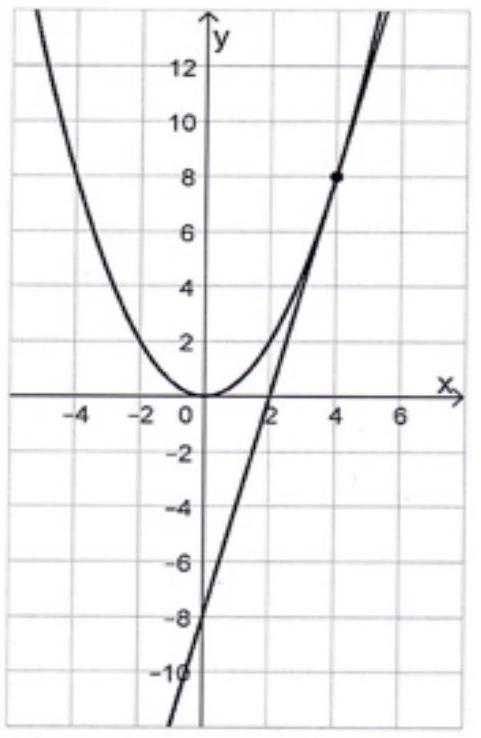
\includegraphics[max width=\textwidth, center]{2025_04_24_9a0606681ee6b3dcd57dg-2}

\section*{Aufgabe W2: (5 BE)}
Die Abbildung zeigt die Graphen einer Funktion $f$ sowie ihrer Umkehrfunktion $\bar{f}$. $F$ ist eine Stammfunktion von f. Die Punkte $P(4 \mid 2)$ und $Q(6 \mid 3)$ liegen auf dem Graphen von $\bar{f}$. Begründen Sie mithilfe geeigneter Eintragungen in der Abbildung, dass der Inhalt der markierten Fläche durch $10-(F(3)-F(2))$ berechnet werden kann.\\
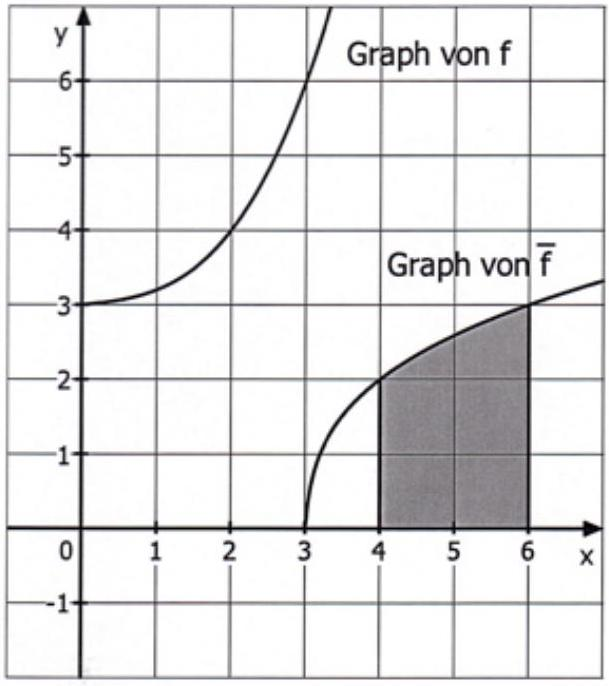
\includegraphics[max width=\textwidth, center]{2025_04_24_9a0606681ee6b3dcd57dg-2(1)}

\section*{Aufgabe W3: (2 BE und 3 BE)}
Die Mittelpunkte der Seitenflächen eines Würfels sind die Eckpunkte eines Oktaeders (vgl. Abbildung). Die Eckpunkte $\mathrm{A}(1|2| 1)$, $\mathrm{B}, \mathrm{C}(-3|-6| 9)$ und D des Oktaeders liegen in der Ebene H mit der Gleichung $2 \mathrm{x}_{1}+\mathrm{x}_{2}+2 \mathrm{x}_{3}=6$.\\
a) Weisen Sie nach, dass die Kantenlänge des Würfels 12 beträgt.\\
b) Bestimmen Sie die Koordinaten eines der beiden Eckpunkte des Oktaeders, die nicht in H liegen.\\
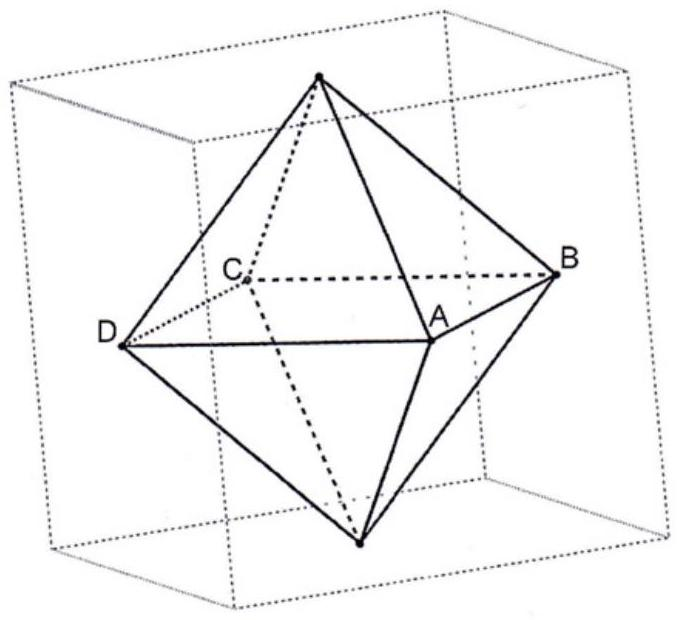
\includegraphics[max width=\textwidth, center]{2025_04_24_9a0606681ee6b3dcd57dg-3}

\section*{Aufgabe W4: (1 BE und 4 BE)}
Gegeben ist die Schar der Geraden $g_{k}: \vec{x}=\left(\begin{array}{c}k \\ -4 k \\ k\end{array}\right)+\mu \cdot\left(\begin{array}{l}4 \\ 8 \\ 1\end{array}\right)$ mit $\mu \in \mathbb{R}$ und $k \in \mathbb{R}$.\\
a) Begründen Sie, dass alle Geraden der Schar parallel zueinander sind.\\
b) Betrachtet wird das Quadrat mit folgenden Eigenschaften:\\
(1) Die Punkte $\mathrm{O}(0|0| 0)$ und $\mathrm{P}(11|4| 5)$ sind Eckpunkte des Quadrats.\\
(2) Zwei Seiten des Quadrats liegen auf Geraden der Schar.

Weisen Sie nach, dass O und P keine benachbarten Eckpunkte dieses Quadrats sind.

\section*{Aufgabe W5: (5 BE)}
Die drei nicht sichtbaren Seiten des abgebildeten Würfels sollen jeweils mit einer der Zahlen 3, 4, 5 oder 6 beschriftet werden. Dabei können Zahlen auch mehrfach verwendet werden.\\
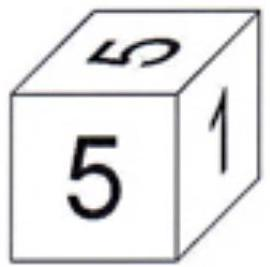
\includegraphics[max width=\textwidth, center]{2025_04_24_9a0606681ee6b3dcd57dg-4}

Nach der Beschriftung soll der Würfel folgende Eigenschaften haben:

\begin{itemize}
  \item Beim einmaligen Werfen ist der Erwartungswert für die erzielte Zahl gleich 4.
  \item Auf den sechs Seiten des Würfels kommen genau drei verschiedene Zahlen vor.
  \item Die Wahrscheinlichkeit dafür, dass beim zweimaligen Werfen des Würfels zweimal die gleiche Zahl erzielt wird, beträgt $\frac{1}{2}$.\\
Untersuchen Sie, ob es möglich ist, die nicht sichtbaren Seiten des Würfels so zu beschriften, dass er alle drei Eigenschaften besitzt.
\end{itemize}

\section*{Aufgabe W6: (5 BE)}
Bei einem Zufallsexperiment gilt für zwei Ereignisse $A$ und $B$ :

\begin{itemize}
  \item $P(A \cap B)=3 x$ mit $x>0$
  \item $P(\bar{A} \cap B)=P(\bar{A} \cap \bar{B})$
  \item $P_{B}(A)=\frac{3}{4}$
\end{itemize}

Stellen Sie den beschriebenen Zusammenhang in einer vollständig ausgefüllten Vierfeldertafel dar und begründen Sie, dass $\mathrm{x} \leq \frac{1}{5}$ gelten muss.

\section*{Aufgabe W1:}
a) Ansatz für die Tangentengleichung: $y=m x+c$\\
y-Achsenabschnitt = c = -8\\
Steigung $\mathrm{m}=4$\\
Tangentengleichung: $y=4 x-8$\\
b) Allgemeine Tangentengleichung an der Stelle $x=u: y=f_{a}^{\prime}(u) \cdot(x-u)+f_{a}(u)$

Es gilt $f_{a}(u)=a \cdot u^{2}$\\
Wegen $f_{a}^{\prime}(x)=2 a x$ gilt $f_{a}^{\prime}(u)=2 a \cdot u$.\\
$y=2 a \cdot u \cdot(x-u)+a \cdot u^{2}$\\
$\Leftrightarrow y=2 a u \cdot x-a \cdot u^{2}$\\
Da der y-Achsenabschnitt der Tangente $-\mathrm{a} \cdot \mathrm{u}^{2}$ ist, schneidet die Tangente die y-Achse im Punkt (0|-a $\cdot \mathrm{u}^{2}$ )

\section*{Aufgabe W2:}
Der Graph der Umkehrfunktion $\bar{f}$ entsteht durch Spiegelung des Graphen von $f$ an der ersten Winkelhalbierenden $y=x$.\\
Somit sind die beiden grau markierten Flächen $A$ und $A^{*}$ gleich groß.\\
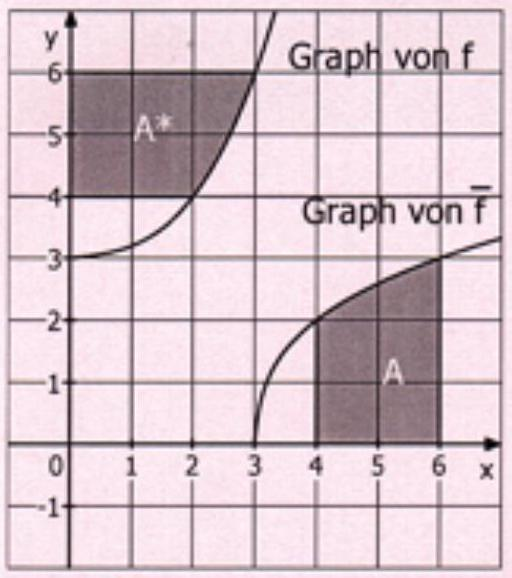
\includegraphics[max width=\textwidth, center]{2025_04_24_9a0606681ee6b3dcd57dg-5}

$$
\begin{aligned}
A & =A^{*}=2 \cdot 2+\int_{2}^{3}(6-f(x)) d x=4+[6 x-F(x)]_{2}^{3}=4+(18-F(3))-(12-F(2)) \\
& =10+F(2)-F(3)=10-(F(3)-F(2))
\end{aligned}
$$

\section*{Aufgabe W3:}
a) Die Kantenlänge des Würfels beträgt $\left.|\overrightarrow{\mathrm{AC}}|=\left(\begin{array}{c}-4 \\ -8 \\ 8\end{array}\right) \right\rvert\,=\sqrt{16+64+64}=\sqrt{144}=12$\\
b) Mittelpunkt der Kante AC: M( $\left.\frac{1-3}{2}\left|\frac{2-6}{2}\right| \frac{1+9}{2}\right)$ bzw. M(-1|-2|5)

Der Abstand von M zur oberen Spitze $S$ des Würfels ist 6 .\\
Zur Berechnung der Koordinaten von S wird der Normaleneinheitsvektor der Ebene H benötigt:

Es gilt $\overrightarrow{\mathrm{n}}=\left(\begin{array}{l}2 \\ 1 \\ 2\end{array}\right)$. Wegen $|\overrightarrow{\mathrm{n}}|=\sqrt{4+1+4}=3$ gilt $\overrightarrow{\mathrm{n}_{0}}=\frac{1}{3} \cdot\left(\begin{array}{l}2 \\ 1 \\ 2\end{array}\right)$.\\
Koordinaten von S: $\overrightarrow{\mathrm{OS}}=\overrightarrow{\mathrm{OM}}+6 \cdot \overrightarrow{\mathrm{n}_{0}}=\left(\begin{array}{c}-1 \\ -2 \\ 5\end{array}\right)+6 \cdot \frac{1}{3} \cdot\left(\begin{array}{l}2 \\ 1 \\ 2\end{array}\right)=\left(\begin{array}{c}-1 \\ -2 \\ 5\end{array}\right)+\left(\begin{array}{l}4 \\ 2 \\ 4\end{array}\right)=\left(\begin{array}{l}3 \\ 0 \\ 9\end{array}\right)$\\
Also gilt $\mathrm{S}(3|0| 9)$.\\
Alternativ kann auch die untere Spitze S* des Würfels berechnet werden.\\
Koordinaten von $\mathrm{S}^{*}: \overrightarrow{\mathrm{OS}^{*}}=\overrightarrow{\mathrm{OM}}-6 \cdot \overrightarrow{\mathrm{n}_{0}}=\left(\begin{array}{c}-1 \\ -2 \\ 5\end{array}\right)-6 \cdot \frac{1}{3} \cdot\left(\begin{array}{l}2 \\ 1 \\ 2\end{array}\right)=\left(\begin{array}{c}-1 \\ -2 \\ 5\end{array}\right)-\left(\begin{array}{l}4 \\ 2 \\ 4\end{array}\right)=\left(\begin{array}{c}-5 \\ -4 \\ 1\end{array}\right)$ Also gilt $S^{*}(-5|-4| 1)$.

\section*{Aufgabe W4:}
a) Alle Geraden sind zueinander parallel, da sie denselben Richtungsvektor besitzen.\\
b)\\
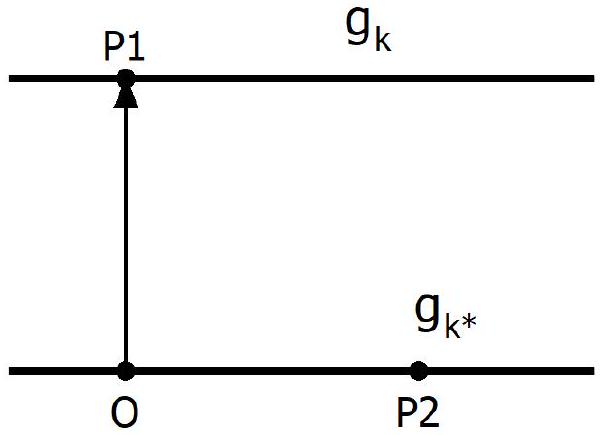
\includegraphics[max width=\textwidth, center]{2025_04_24_9a0606681ee6b3dcd57dg-7}

Wenn der Punkt P ein benachbarter Punkt von O ist gibt es zwei Möglichkeiten:\\
1.Möglichkeit:

Die Punkte O und P (in der Zeichnung mit P1 bezeichnet) liegen auf zwei unterschiedlichen Geraden der Schar.\\
Dies ist der Fall, wenn der Vektor $\overrightarrow{\mathrm{OP}}$ und der Richtungsvektor der Gerade orthogonal zueinander sind.\\
Da $\left(\begin{array}{c}11 \\ 4 \\ 5\end{array}\right) \cdot\left(\begin{array}{l}4 \\ 8 \\ 1\end{array}\right)=44+32+5=81 \neq 0$ ist, sind die Vektoren nicht orthogonal zueinander, also scheidet die 1.Möglichkeit aus.\\
2.Möglichkeit:

Die Punkte O und P (in der Zeichnung mit P2 bezeichnet) liegen auf derselben Schargerade.

Einsetzen des Punktes $\mathrm{O}(0|0| 0)$ in die Schargerade:\\
$\left(\begin{array}{l}0 \\ 0 \\ 0\end{array}\right)=\left(\begin{array}{c}k \\ -4 \mathrm{k} \\ \mathrm{k}\end{array}\right)+\mu \cdot\left(\begin{array}{l}4 \\ 8 \\ 1\end{array}\right) \quad \begin{aligned} 0 & =\mathrm{k}+4 \mu \\ 0 & =-4 \mathrm{k}+8 \mu \\ 0 & =\mathrm{k}+\mu\end{aligned}$\\
Zeile (1) - Zeile (3): $0=3 \mu \Leftrightarrow \mu=0$\\
Einsetzen in Zeile ergibt $\mathrm{k}=0$.\\
Der Ursprung O liegt auf der Gerade $g_{0}: \vec{x}=\left(\begin{array}{l}0 \\ 0 \\ 0\end{array}\right)+\mu \cdot\left(\begin{array}{l}4 \\ 8 \\ 1\end{array}\right)$

Kontrolle, ob der Punkt $P(11|4| 5)$ auf $g_{0}$ liegt:

$$
\left(\begin{array}{l}
11 \\
4 \\
5
\end{array}\right)=\left(\begin{array}{l}
0 \\
0 \\
0
\end{array}\right)+\mu \cdot\left(\begin{array}{l}
4 \\
8 \\
1
\end{array}\right)
$$

Aus Zeile (3) folgt $\mu=5$\\
Aus Zeile (2) folgt $\mu=0,5$.\\
Daher liegt $P$ nicht auf $g_{0}$.\\
Damit scheidet auch die Möglichkeit 2 aus.\\
Somit sind O und P keine benachbarten Eckpunkte des Quadrats.

\section*{Aufgabe W5:}
Die fehlenden Augenzahlen werden mit x und y und z bezeichnet.\\
Der Erwartungswert der Augenzahlen beträgt 4.

$$
\begin{aligned}
\text { Erwartungswert }=\frac{1}{6} x+\frac{1}{6} y & +\frac{1}{6} z+\frac{1}{6} \cdot 1+\frac{2}{6} \cdot 5=4 \\
& \left.\Leftrightarrow \frac{1}{6} x+\frac{1}{6} y+\frac{1}{6} z=\frac{13}{6} \quad \right\rvert\, \cdot 6 \\
& \Leftrightarrow x+y+z=13
\end{aligned}
$$

Da auf dem Würfel insgesamt nur 3 verschiedene Zahlen vorkommen, gibt es nur folgende Möglichkeiten der Beschriftung, die die obige Gleichung erfüllen:

Fall 1: $x=3$ und $y=z=5$\\
Fall 2: $x=5$ und $y=z=4$\\
Fall1 : $\mathrm{P}($ zweimal dieselbe Zahl bei zweimaligem Würfeln $)=\mathrm{P}(11,33,55)$

$$
=\frac{1}{36}+\frac{1}{36}+\frac{16}{36}=\frac{1}{2}
$$

Fall 2: $P($ zweimal dieselbe Zahl bei zweimaligem Würfeln $)=P(11,44,55)$

$$
=\frac{1}{36}+\frac{4}{36}+\frac{9}{36}=\frac{14}{36}=\frac{7}{18}
$$

Da nur Fall 1 die letzte Bedingung erfüllt, ist folgende Würfelbeschriftung für die unsichtbaren drei Würfelseiten möglich:\\
Einmal die Augenzahl „3" und zweimal die Augenzahl „5".

\section*{Aufgabe W6:}
Ansatz Vierfeldertafel:

\begin{center}
\begin{tabular}{|c|c|c|c|}
\hline
 & $B$ & $\bar{B}$ &  \\
\hline
$A$ & $3 x$ & $1-5 x$ & $1-2 x$ \\
\hline
$\bar{A}$ & $x$ & $x$ & $2 x$ \\
\hline
 & $4 x$ & $1-4 x$ & 1 \\
\hline
\end{tabular}
\end{center}

$P_{B}(A)=\frac{3}{4} \Leftrightarrow \frac{P(A \cap B)}{P(B)}=\frac{3}{4} \Leftrightarrow \frac{3 x}{P(B)}=\frac{3}{4} \Leftrightarrow P(B)=4 x$\\
Daraus folgt $P(\bar{A} \cap B)=P(B)-P(A \cap B)=4 x-3 x=x$\\
$P(\bar{A} \cap B)=P(\bar{A} \cap \bar{B})=x$\\
Die roten Werte ergeben sich durch Addition und Subtraktion der Zeilen und Spalten aufgrund der schwarzen eingetragenen Werte.

Da $P(A \cap \bar{B})=1-5 x \geq 0$ gelten muss folgt daraus $x \leq \frac{1}{5}$.


\end{document}